\chapter{Resultaten leerproces LDA}
\label{app:LDA}
Deze bijlage bevat een aantal voorbeelden van resultaten van het LDA-leerproces. Het betreft foto's uit de trainingsset met de vijf meest waarschijnlijke topics voor die foto. Deze resultaten zijn ``correct'', aangezien ze uit de trainingsset komen en het model gemodelleerd is op deze data.

\begin{figure}[h]
	\centering
	\begin{minipage}[t]{.5\linewidth}
		\centering
		\vspace{0pt}
		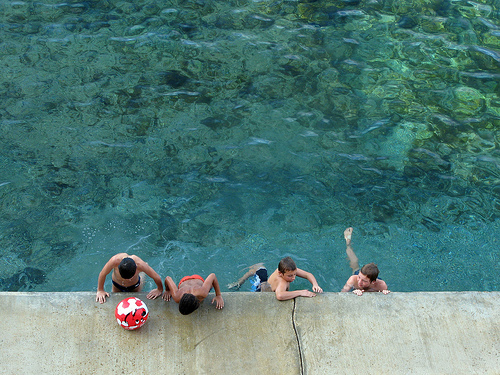
\includegraphics[width=\textwidth]{Images/LDA/3283626303.jpg}
	\end{minipage}\hfill
	\begin{minipage}[t]{.5\textwidth}
		\centering
		\vspace{0pt}
		\begin{tabularx}{\textwidth}{cl}
			topic                           & waarschijnlijkheid\\
			\hline
			\texttt{wall/grafitti} & 0,145\\
			\texttt{pool} & 0,121\\
			\texttt{rock climbing} & 0,098\\
			\texttt{boy} & 0,098\\
			\texttt{body of water} & 0,098\\
			\hline
		\end{tabularx}
	\end{minipage}
	\caption{Afbeelding met de vijf meest waarschijnlijke onderwerpen}
\end{figure}


\begin{figure}
\begin{subfigure}{\textwidth}
    \centering
    \begin{minipage}[t][3.5cm]{.5\linewidth}
    \centering
    \vspace{0pt}
    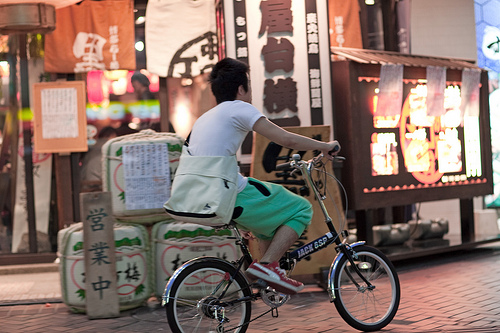
\includegraphics[height=3.5cm]{Images/LDA/4756089621.jpg}
    \end{minipage}\hfill
    \begin{minipage}[t][3.5cm]{.5\textwidth}
    \centering
    \vspace{0pt}
    \begin{tabularx}{\textwidth}{cl}
            topic                           & waarschijnlijkheid\\
            \hline
            \texttt{bicycle }                        &  0,206\\
            \texttt{clothing}                        &  0,124\\
            \begin{tabular}{c}
                \texttt{smile/asian/}\\
                \texttt{camera}
            \end{tabular}            &  0,084\\
            \texttt{shirt/color}                     &  0,084\\
            \texttt{backpack/bag}                    &  0,063\\
            \hline
        \end{tabularx}
    \end{minipage}
\end{subfigure}

\vspace*{4mm}

\begin{subfigure}{\textwidth}
    \centering
    \begin{minipage}[t][3.5cm]{.5\linewidth}
    \centering
    \vspace{0pt}
    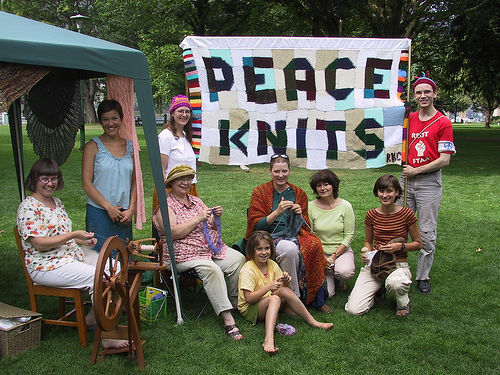
\includegraphics[height=3.5cm]{Images/LDA/4386588.jpg}
    \end{minipage}\hfill
    \begin{minipage}[t][3.5cm]{.5\textwidth}
    \centering
    \vspace{0pt}
    \begin{tabularx}{\textwidth}{cl}
            topic                           & waarschijnlijkheid\\
            \hline
            \texttt{(protest) sign} & 0,293\\
            \texttt{group} & 0,184\\
            \texttt{work} & 0,093\\
            \texttt{clothes+color} & 0,056\\
            \texttt{sit/chair} & 0,038\\
            \hline
        \end{tabularx}
    \end{minipage}
\end{subfigure}

\vspace*{4mm}

\begin{subfigure}{\textwidth}
    \centering
    \begin{minipage}[t][4.5cm]{.5\linewidth}
    \centering
    \vspace{0pt}
    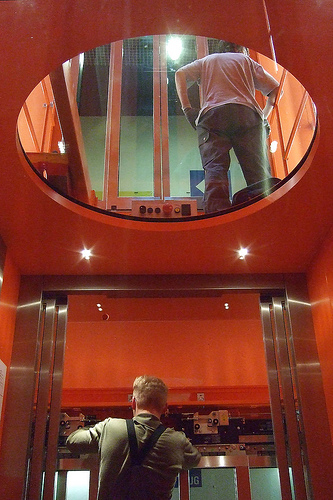
\includegraphics[height=4.5cm]{Images/LDA/2506703854.jpg}
    \end{minipage}\hfill
    \begin{minipage}[t][4.5cm]{.5\textwidth}
    \centering
    \vspace{0pt}
    \begin{tabularx}{\textwidth}{cl}
            topic                           & waarschijnlijkheid\\
            \hline
            \texttt{constructor} & 0,158\\
            \begin{tabular}{c}
                \texttt{computer/}\\
                \texttt{microscope}
            \end{tabular} & 0,113\\
            \begin{tabular}{c}
                \texttt{red/yellow/orange}\\
                \texttt{bright clothing}
            \end{tabular} & 0,113\\
            \texttt{clothes+color} & 0,113\\
            \texttt{sit/chair} & 0,047\\
            \hline
        \end{tabularx}
    \end{minipage}
\end{subfigure}

\vspace*{4mm}

\begin{subfigure}{\textwidth}
    \centering
    \begin{minipage}[t][4.5cm]{.5\linewidth}
    \centering
    \vspace{0pt}
    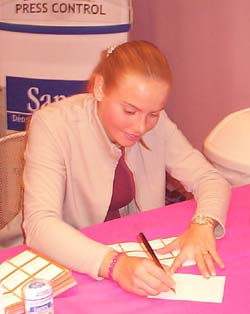
\includegraphics[height=4.5cm]{Images/LDA/23012579.jpg}
    \end{minipage}\hfill
    \begin{minipage}[t][4.5cm]{.5\textwidth}
    \centering
    \vspace{0pt}
    \begin{tabularx}{\textwidth}{cl}
            topic                           & waarschijnlijkheid\\
            \hline
            \texttt{reading/classroom} & 0,282\\
            \texttt{woman/girl} & 0,125\\
            \texttt{jackets} & 0,089\\
            \begin{tabular}{c}
                \texttt{sit at table}\\
                \texttt{restaurant}
            \end{tabular} & 0,089\\
            \texttt{formal clothing} & 0,072\\
            \hline
        \end{tabularx}
    \end{minipage}
\end{subfigure}
\caption{Afbeeldingen met hun vijf meest waarschijnlijke onderwerpen}
\end{figure}

